\subsection{Performance}


\begin{figure*}[ht]

  \begin{subfigure}[b]{0.5\textwidth}
      \centering
      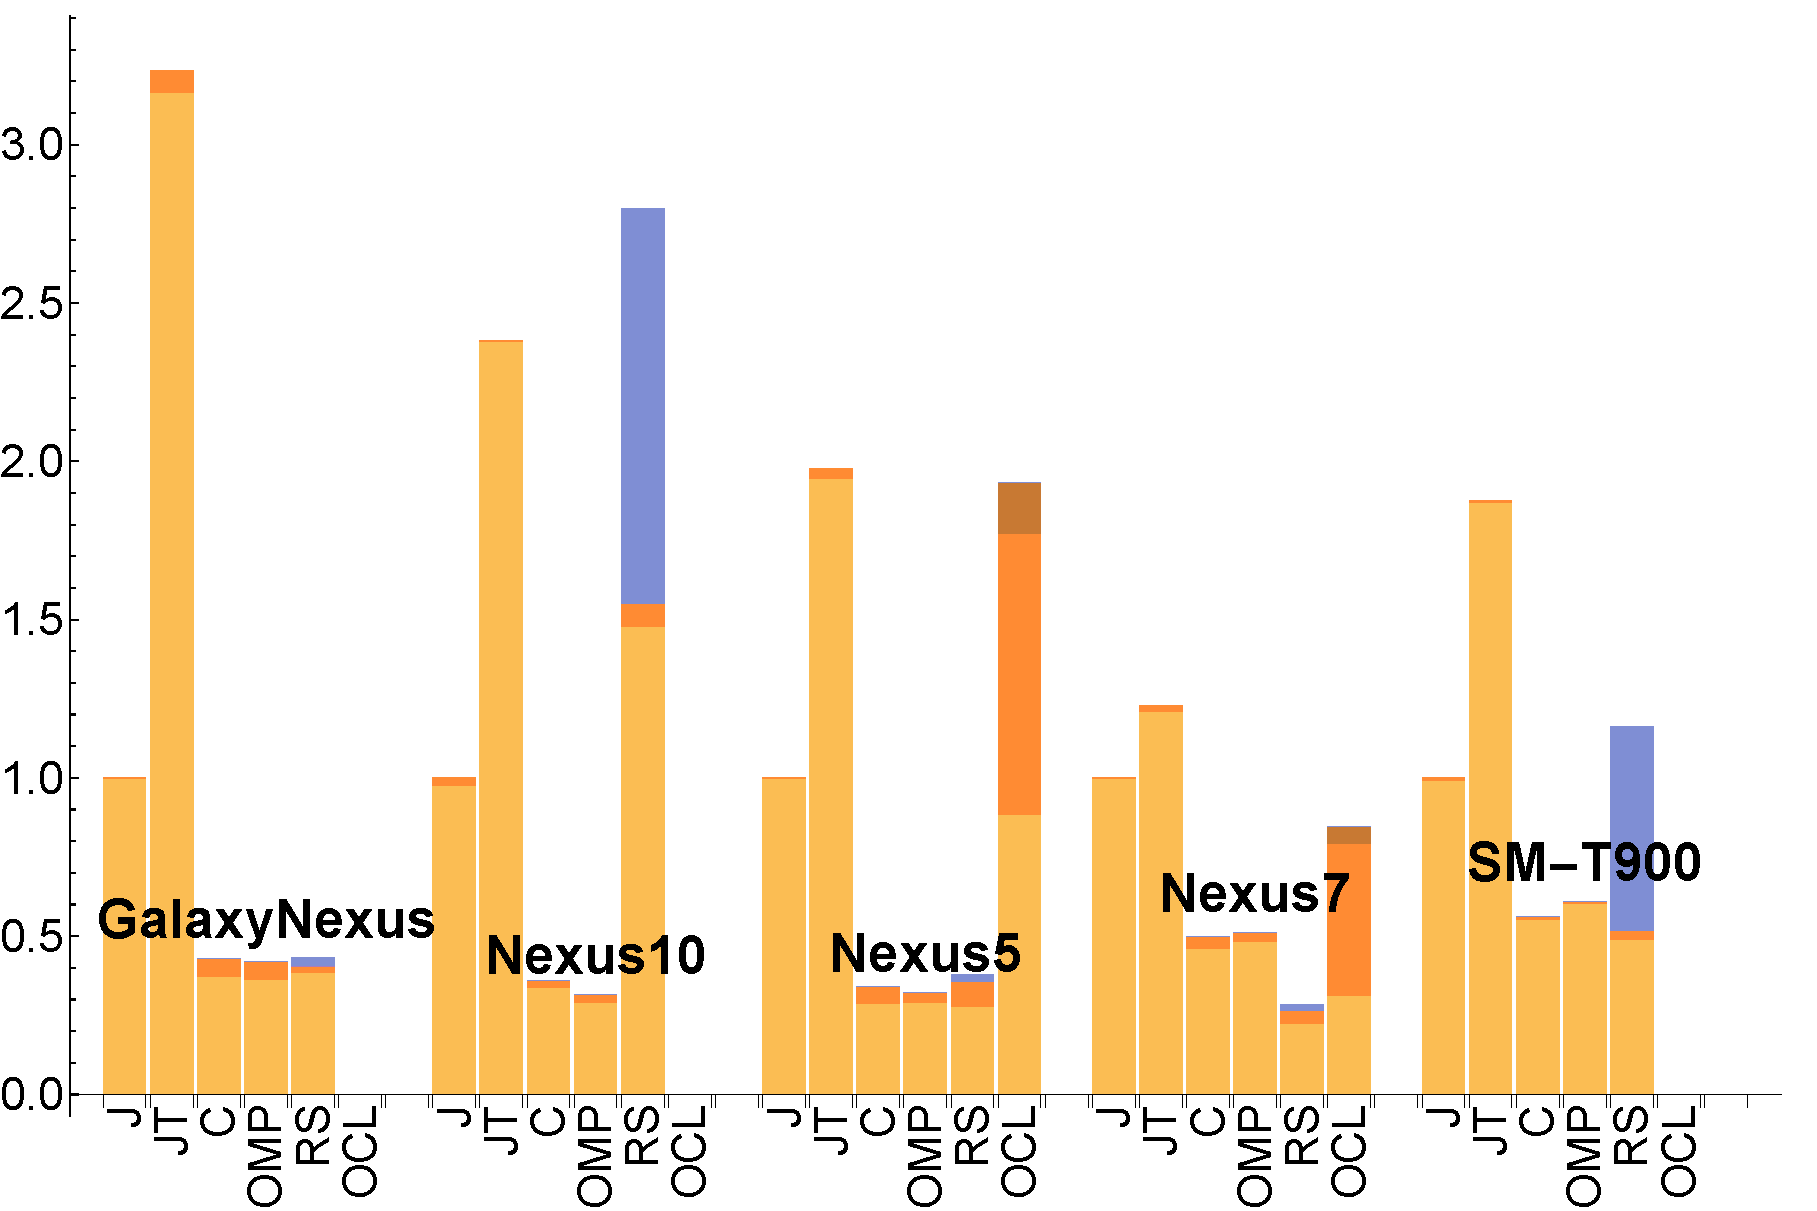
\includegraphics[width=\textwidth]{data/VectorAdd_time.pdf}
      \caption{VectorAdd}\label{fig:vectoradd}
  \end{subfigure}
  \begin{subfigure}[b]{0.5\textwidth}
      \centering
      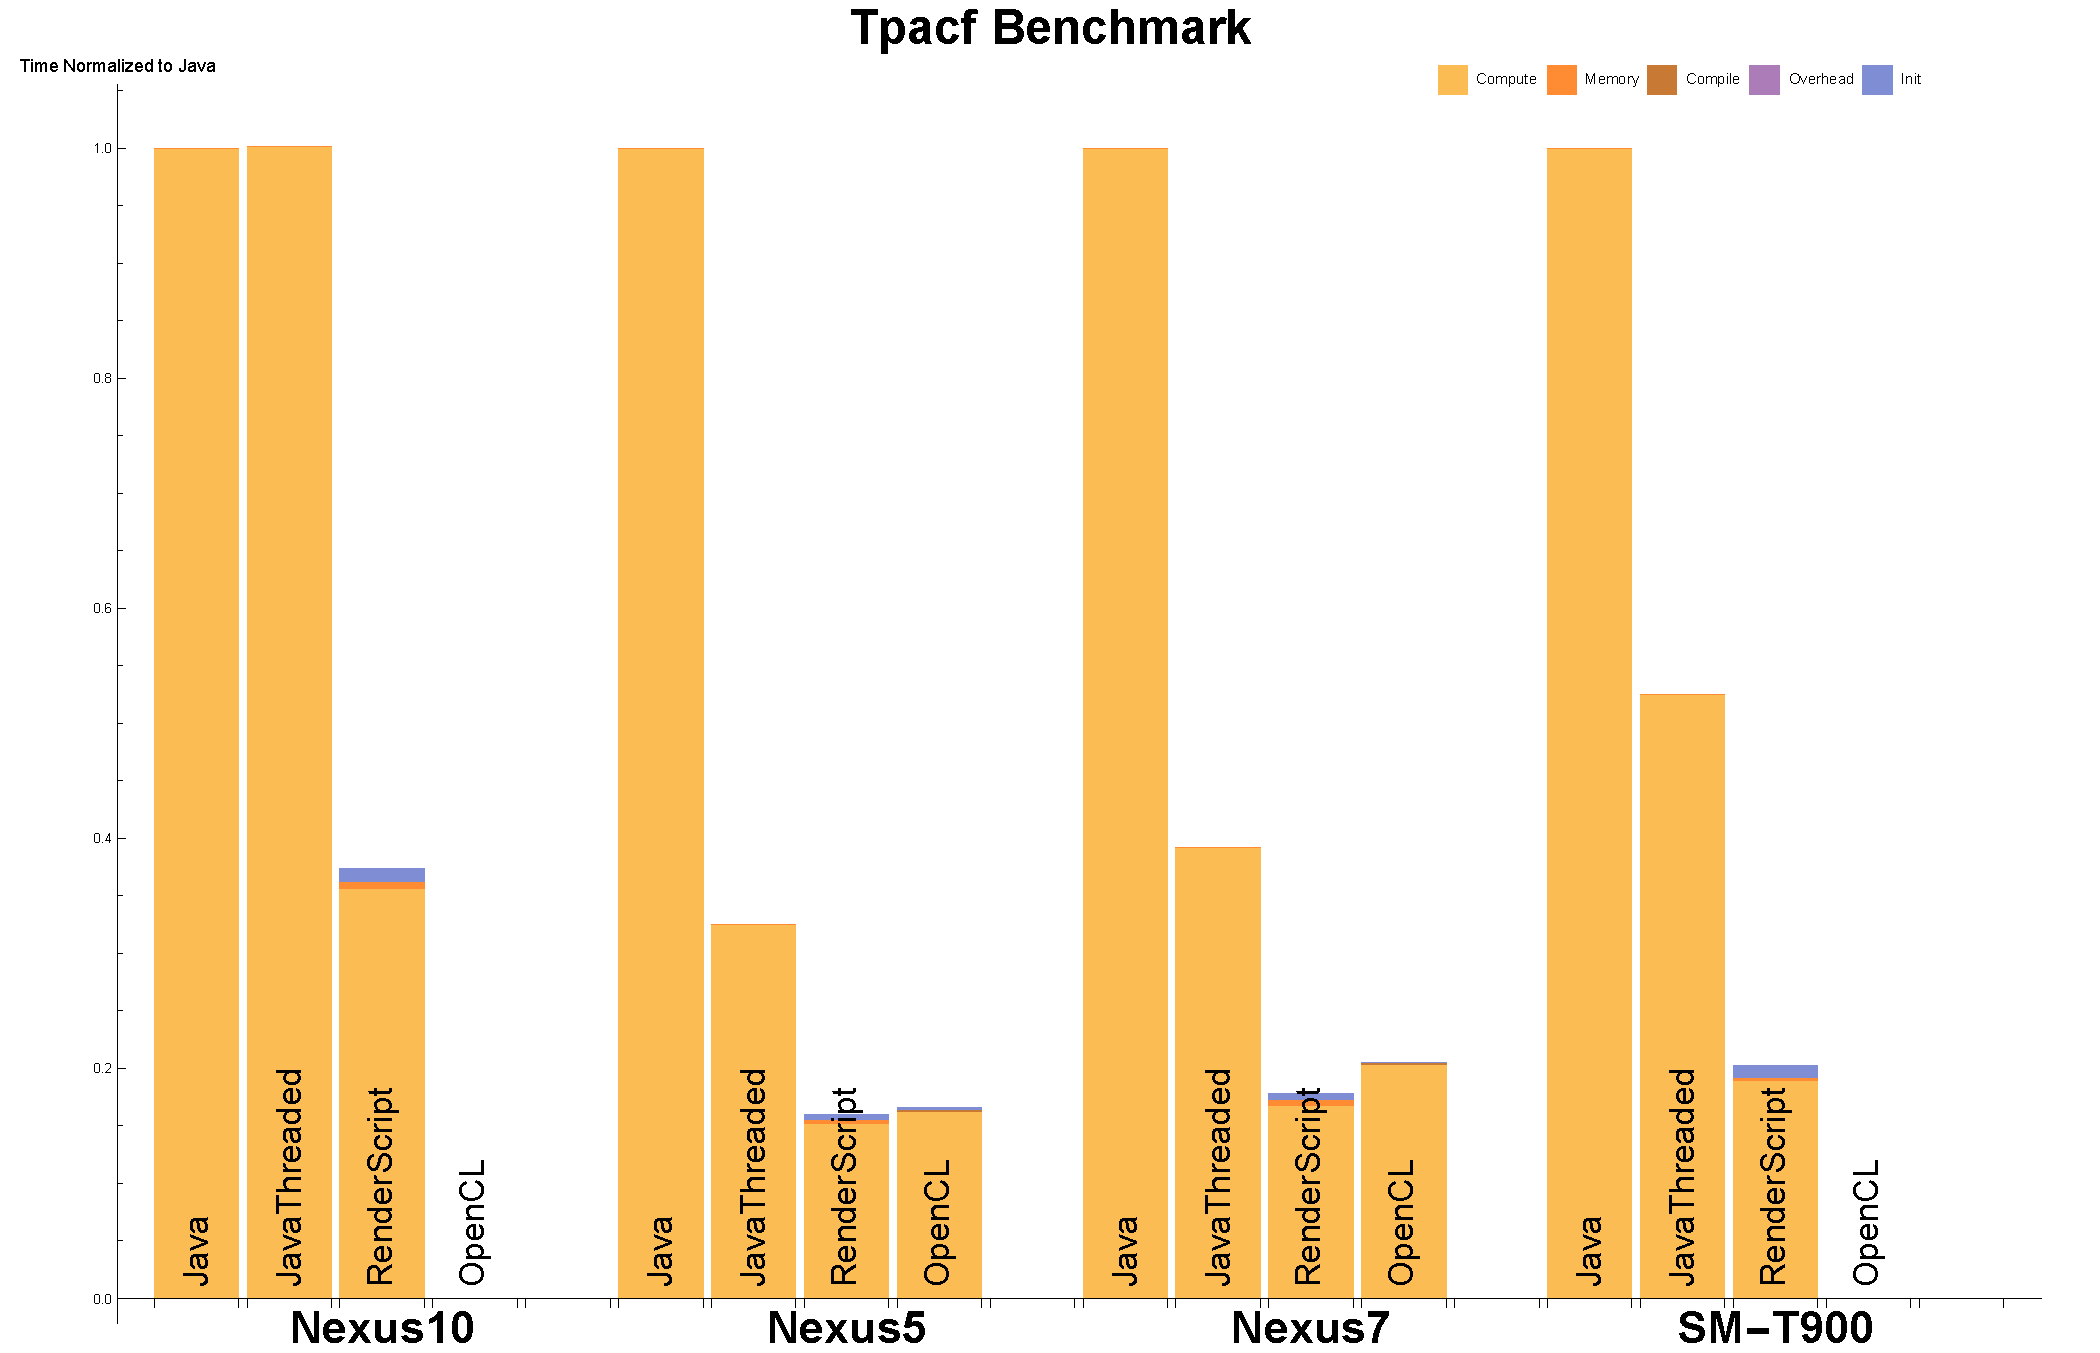
\includegraphics[width=\textwidth]{data/Tpacf_time.pdf}
      \caption{TPACF}
      \label{fig:TPACF}
  \end{subfigure}

  \begin{subfigure}[b]{0.5\textwidth}
      \centering
      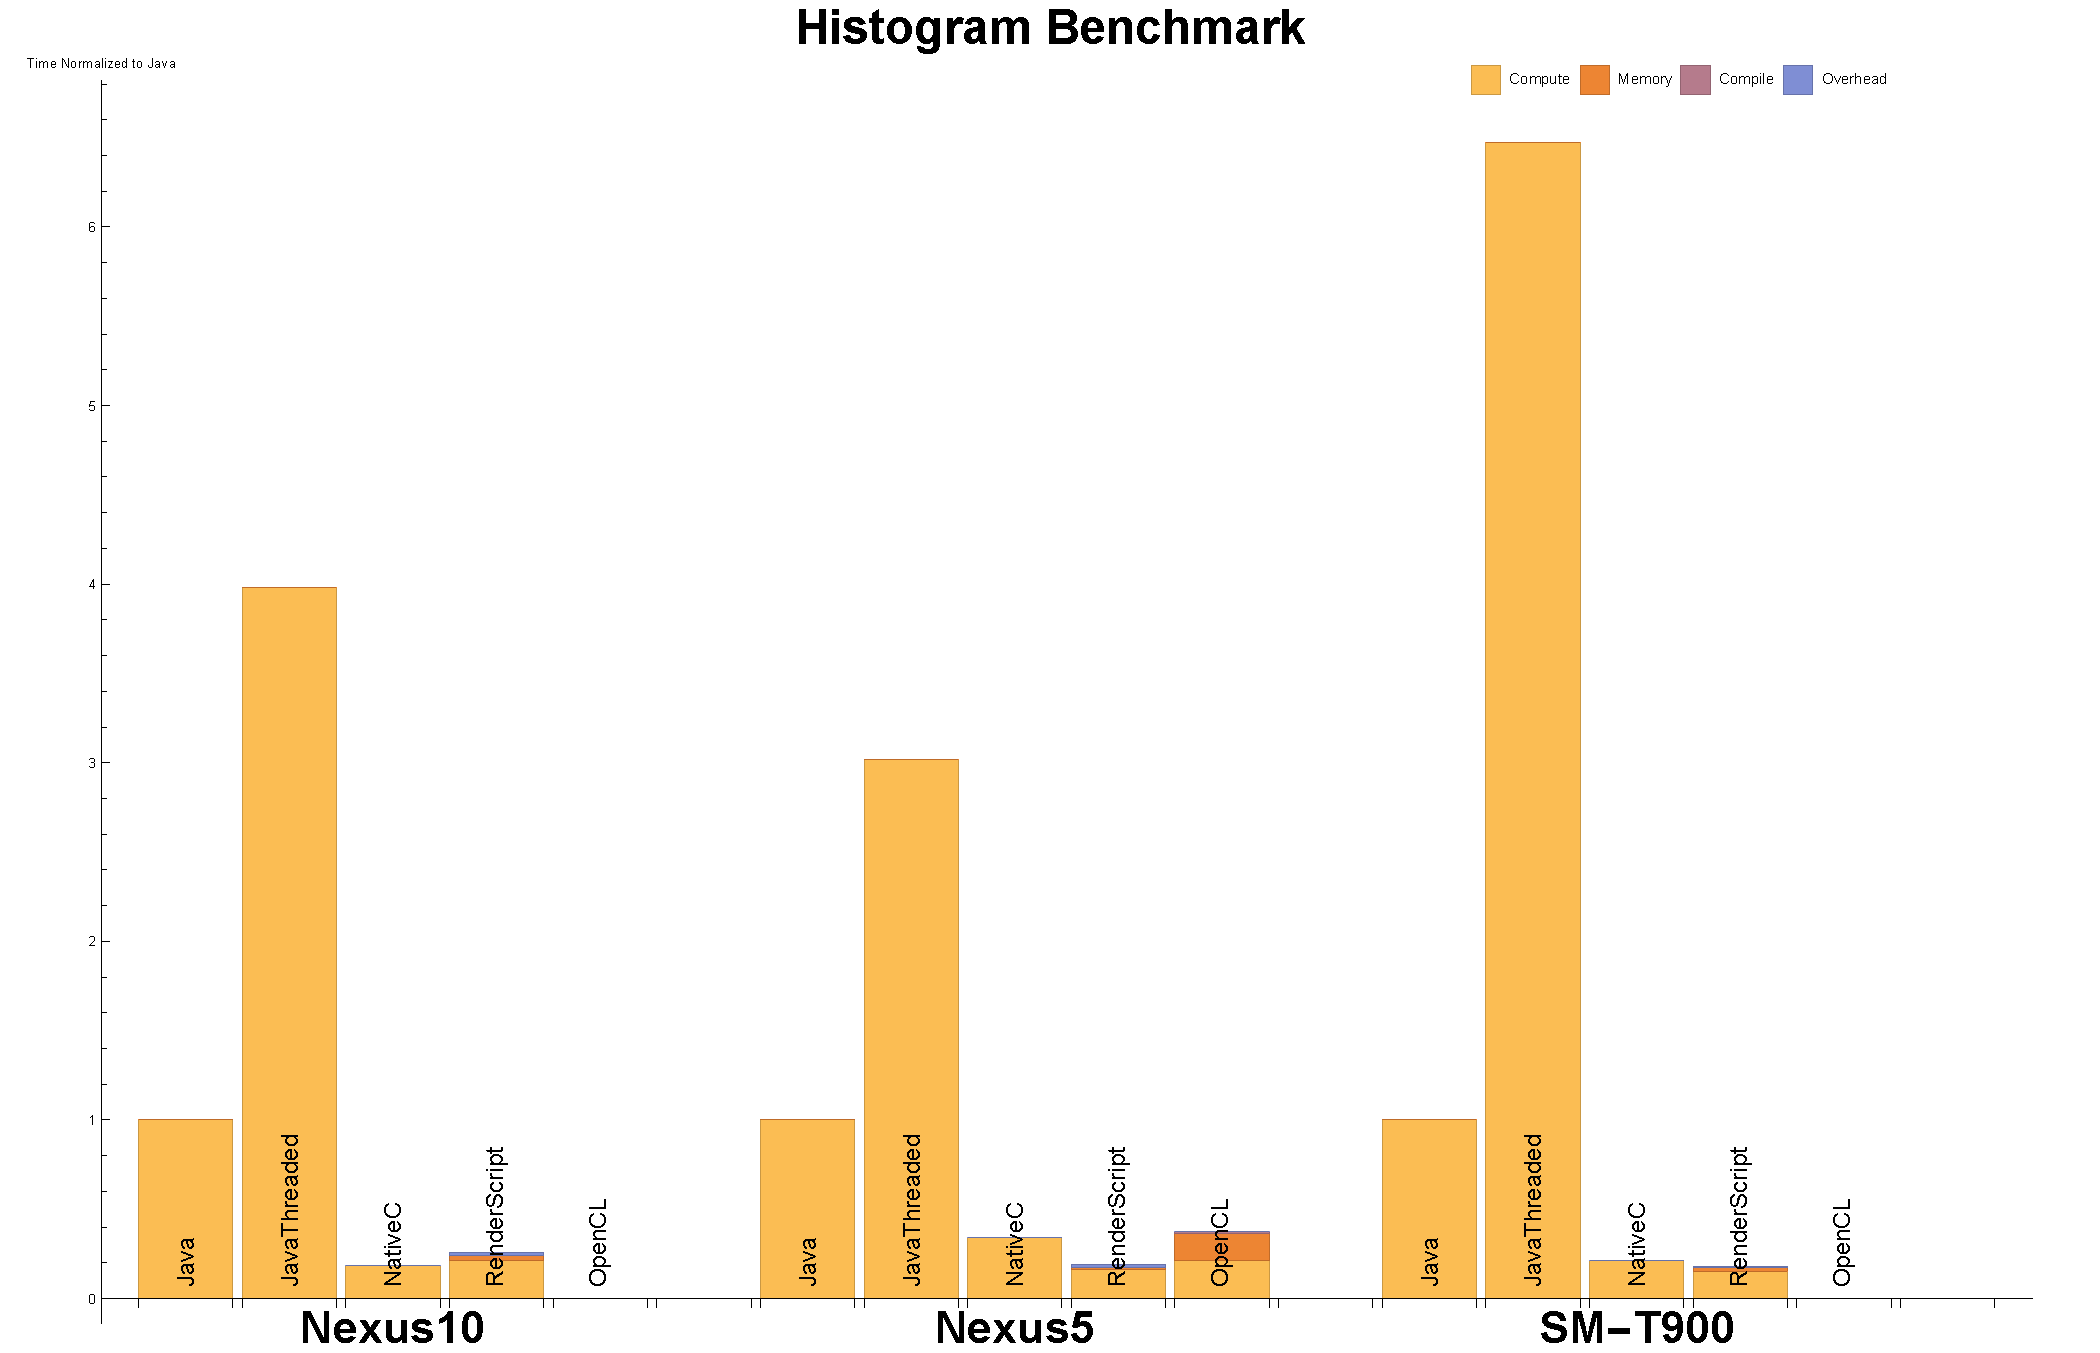
\includegraphics[width=\textwidth]{data/Histogram_time.pdf}
      \caption{Histo}\label{fig:histo}
  \end{subfigure}
  \begin{subfigure}[b]{0.5\textwidth}
      \centering
      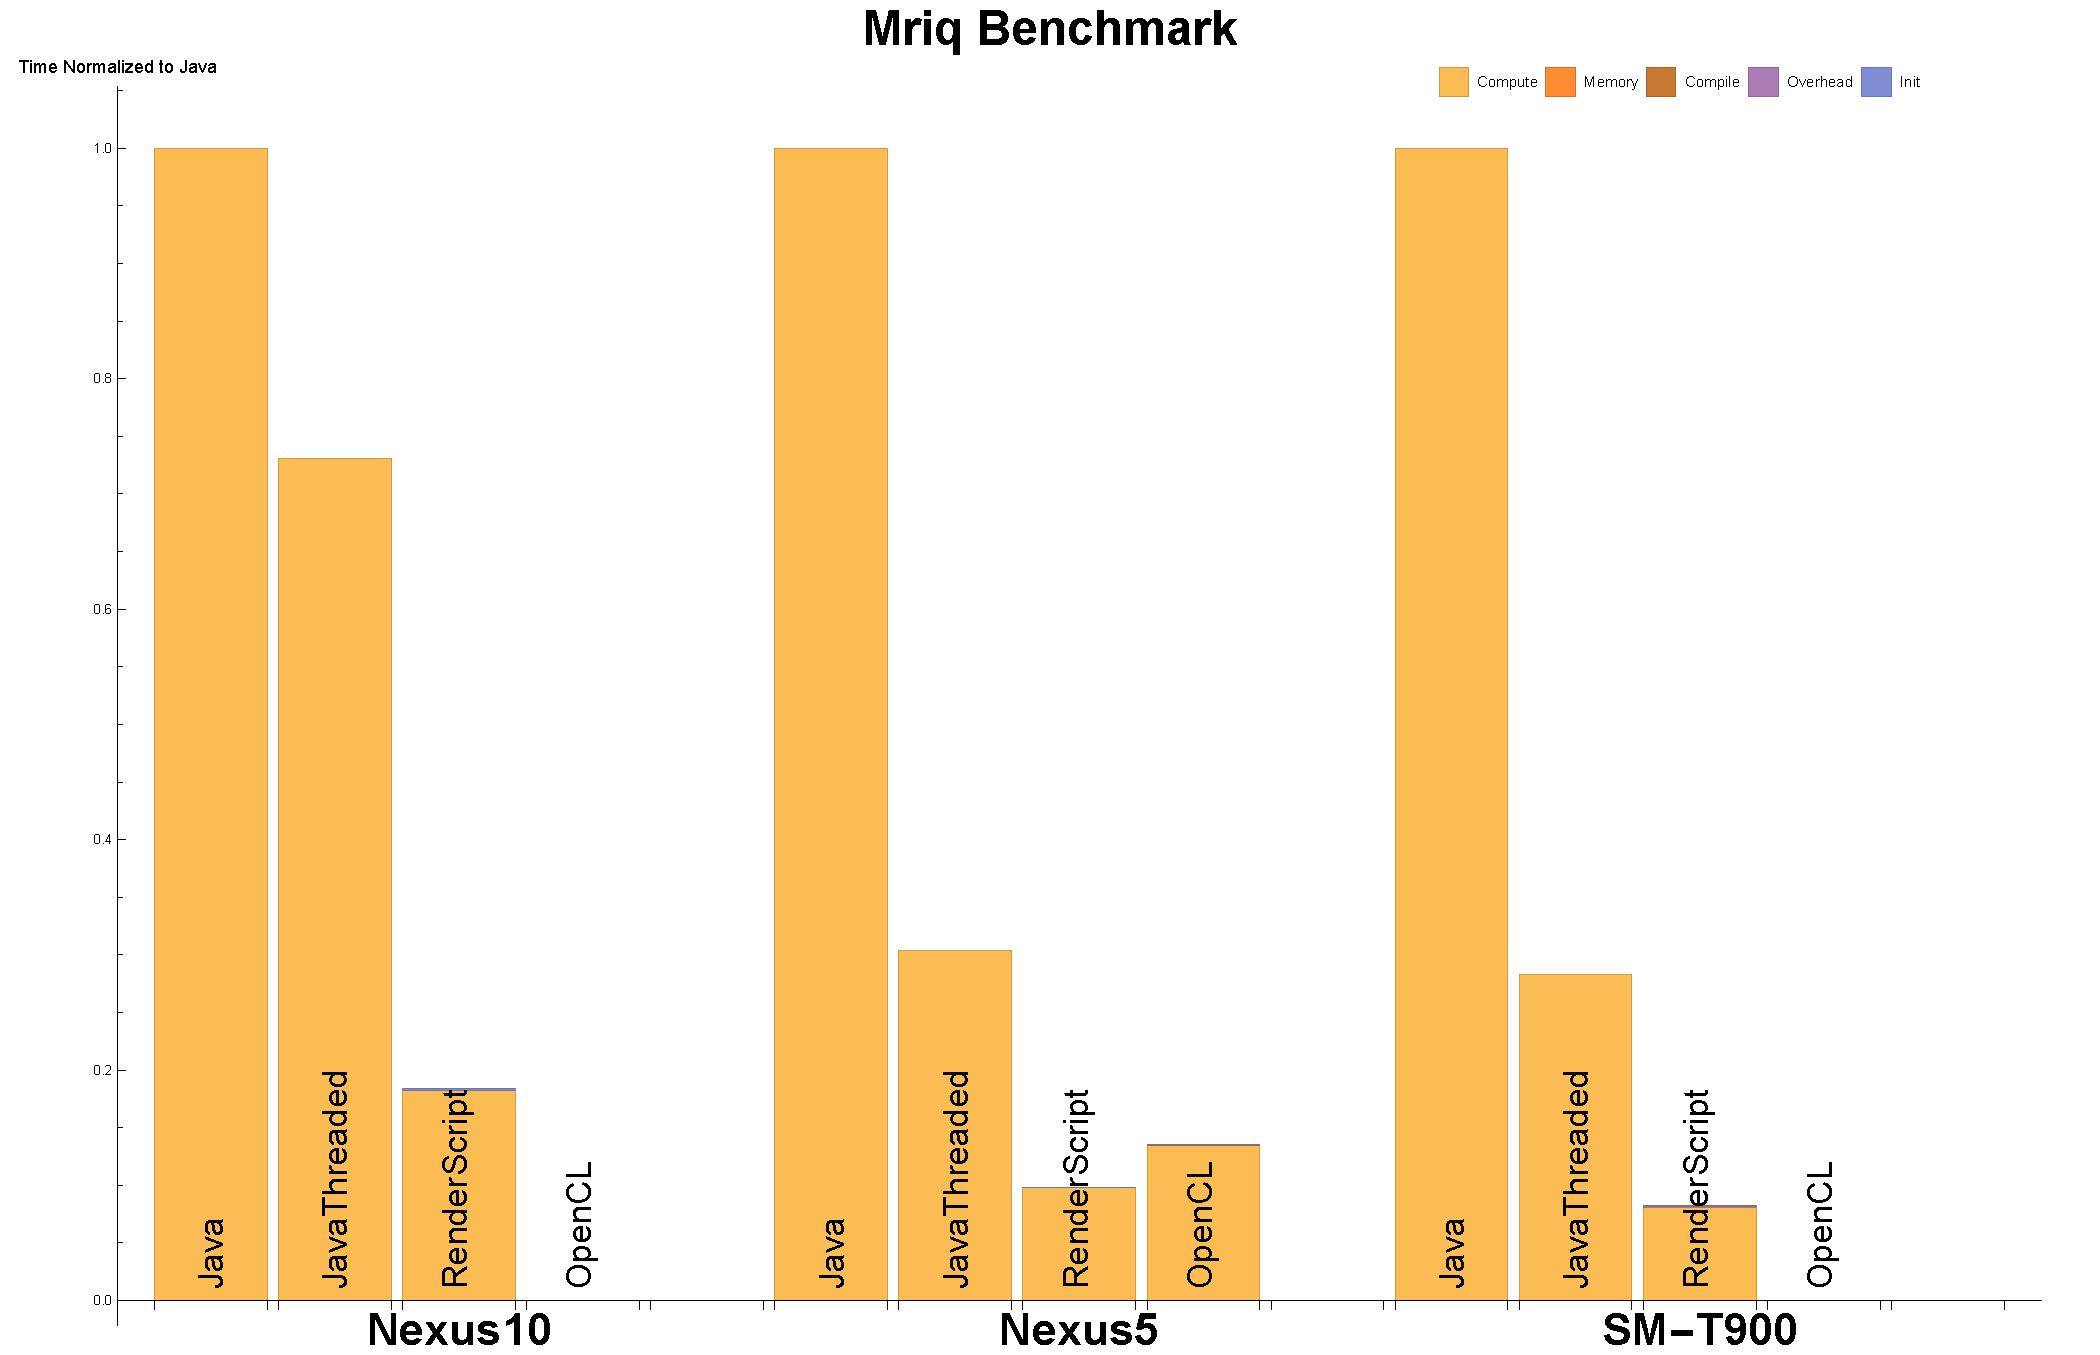
\includegraphics[width=\textwidth]{data/Mriq_time.pdf}
      \caption{MRIQ}
      \label{fig:MRIQ}
  \end{subfigure}

  \begin{subfigure}[b]{0.5\textwidth}
      \centering
      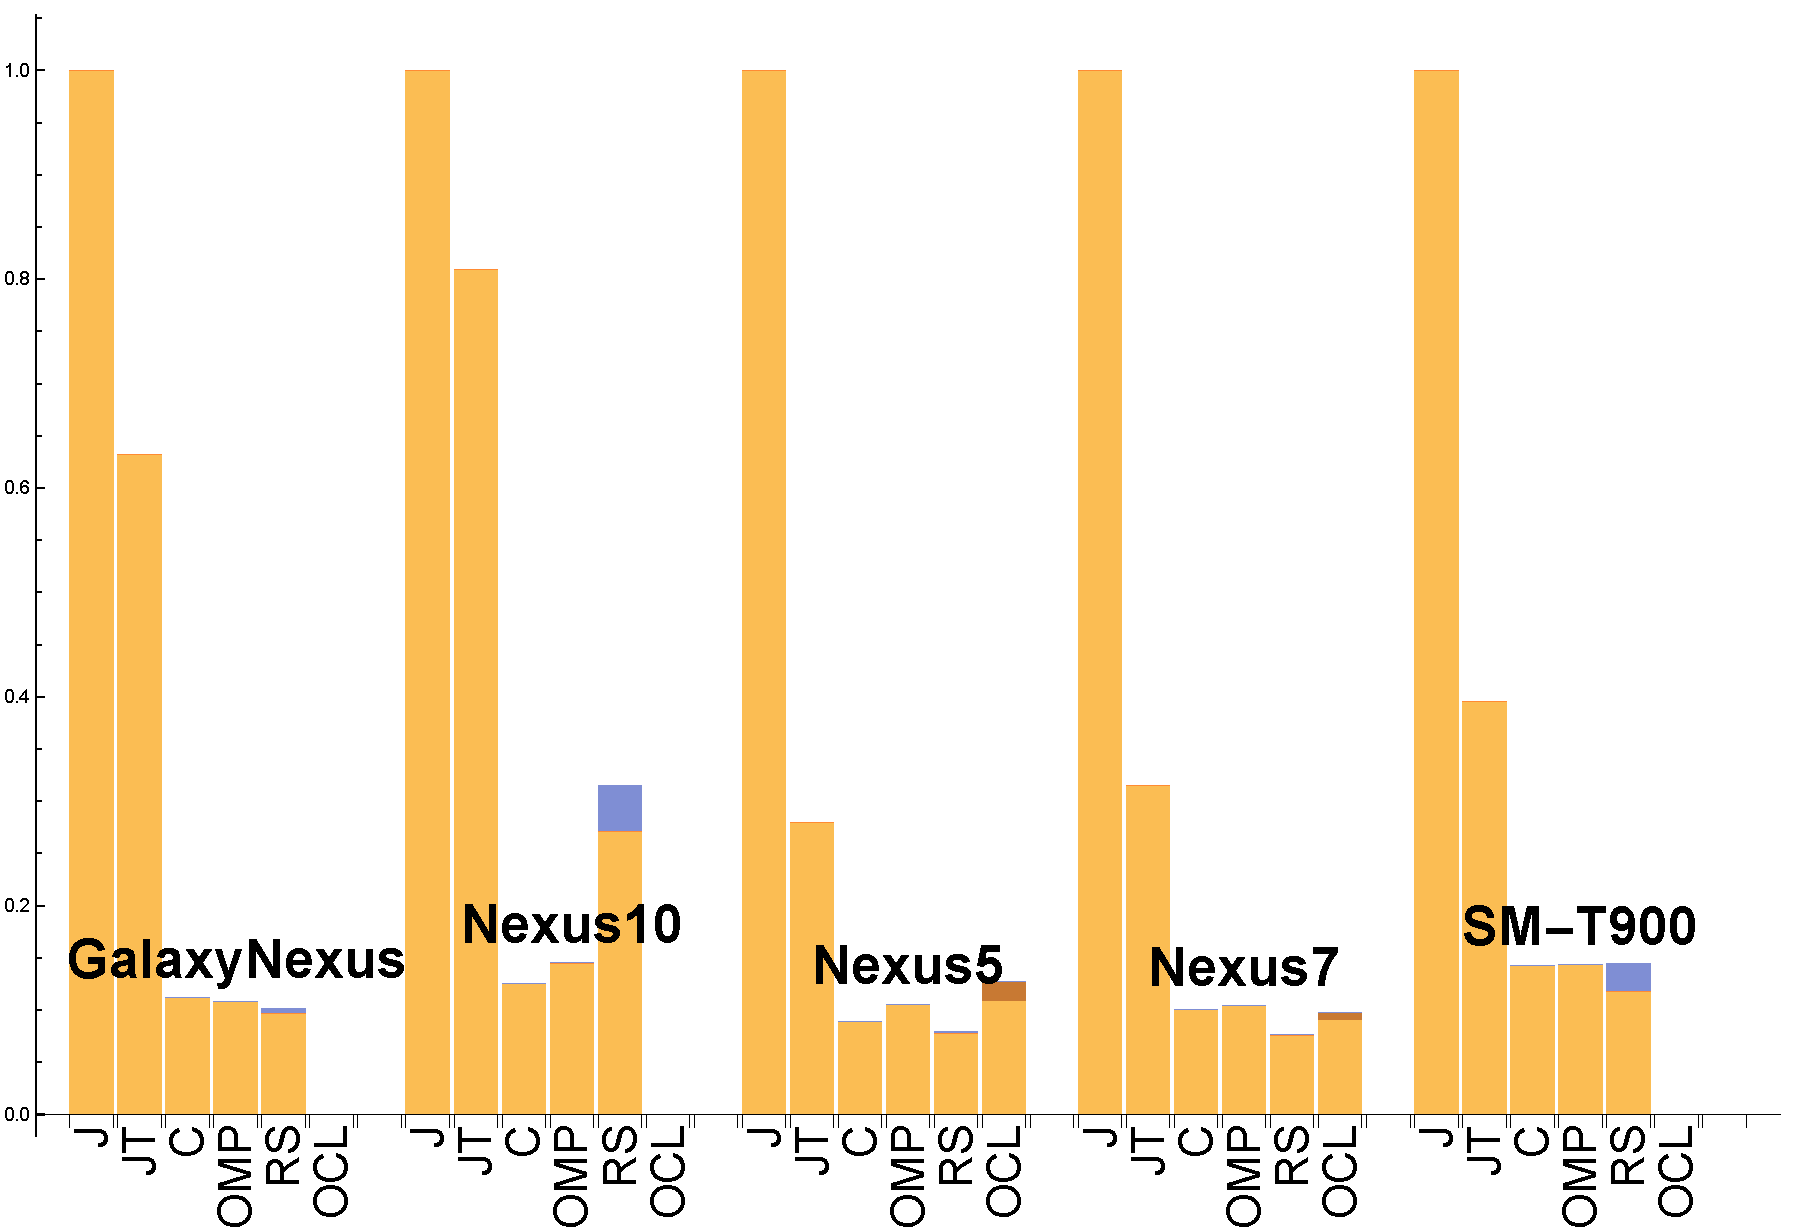
\includegraphics[width=\textwidth]{data/Sgemm_time.pdf}
      \caption{Sgemm}\label{fig:Sgemm}
  \end{subfigure}
  \begin{subfigure}[b]{0.5\textwidth}
      \centering
      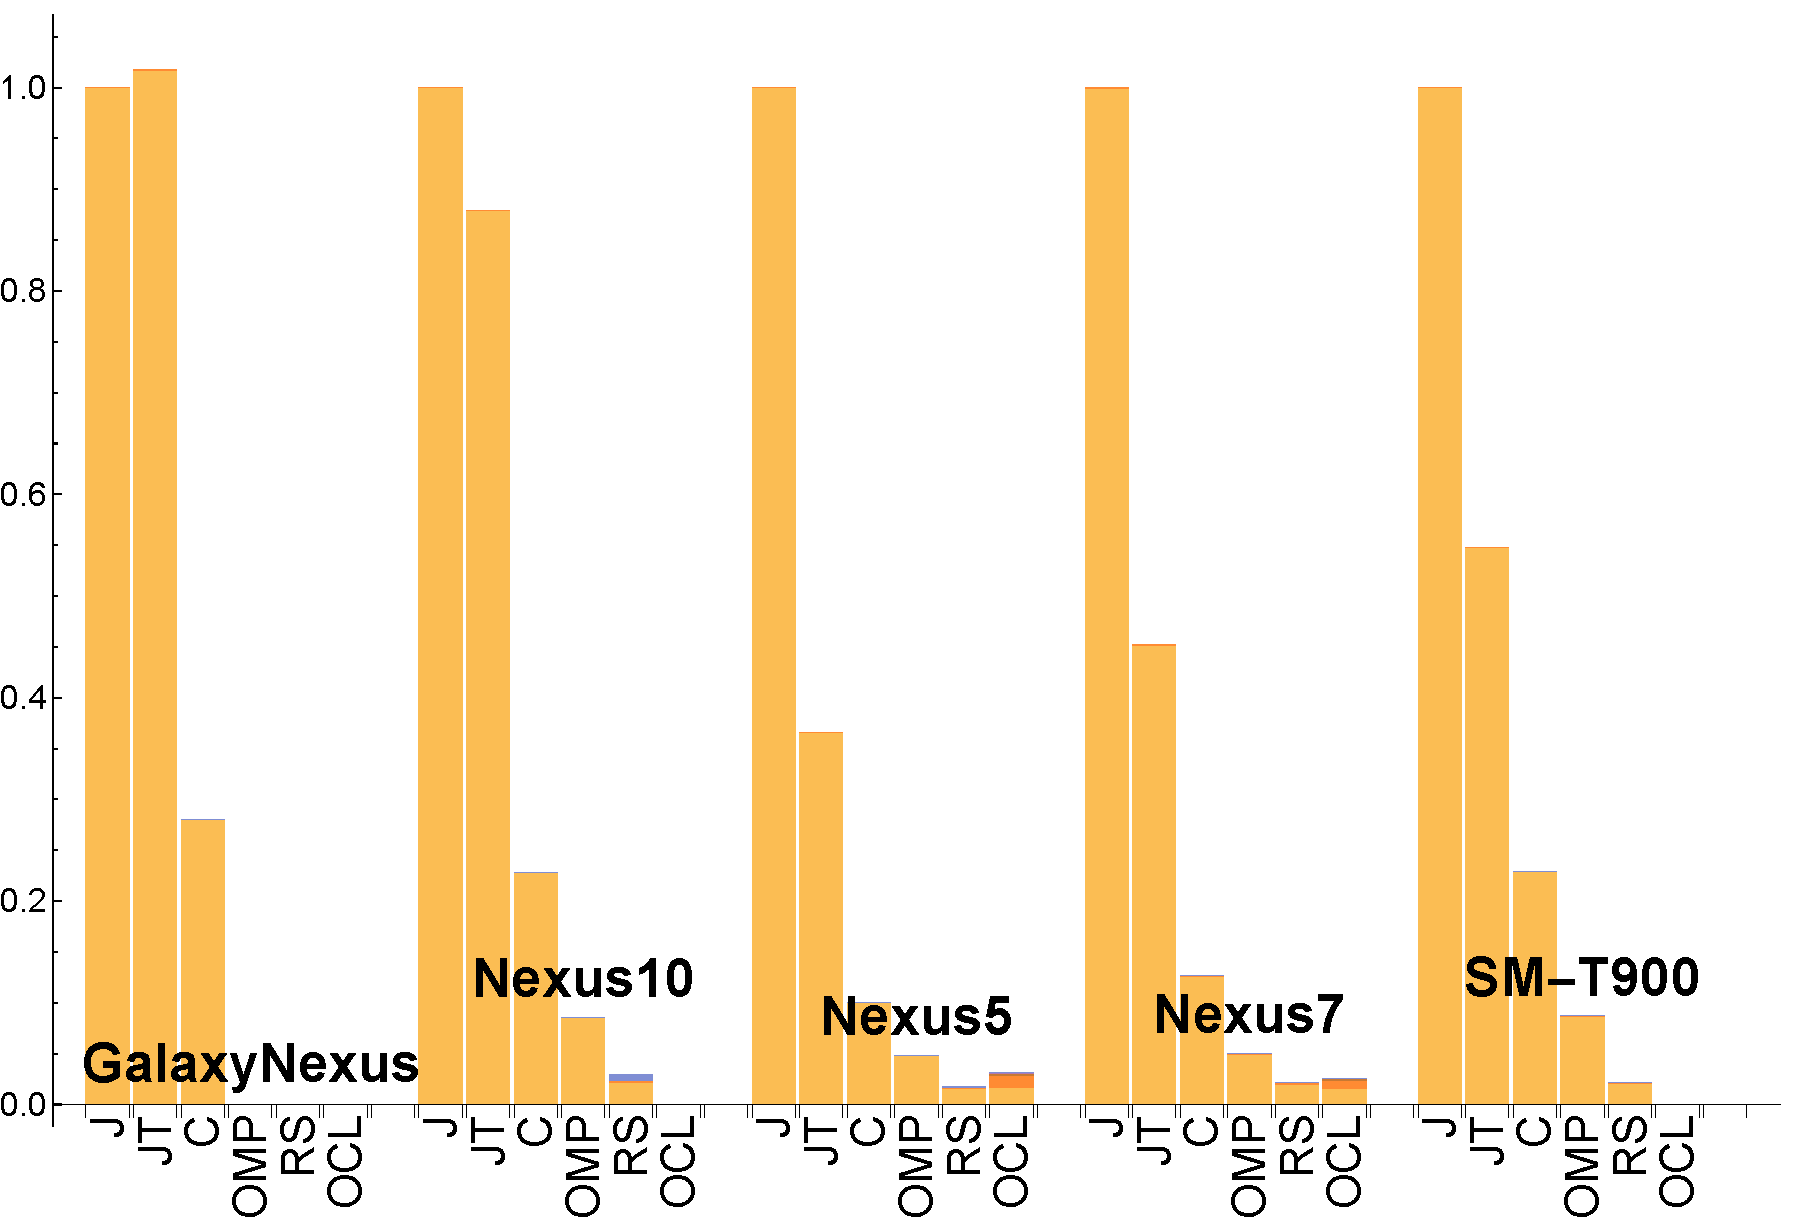
\includegraphics[width=\textwidth]{data/Stencil_time.pdf}
      \caption{Stencil}
      \label{fig:Stencil}
  \end{subfigure}

  \caption{Runtime}
\end{figure*}


\begin{figure*}[ht]

  \begin{subfigure}[b]{0.5\textwidth}
      \centering
      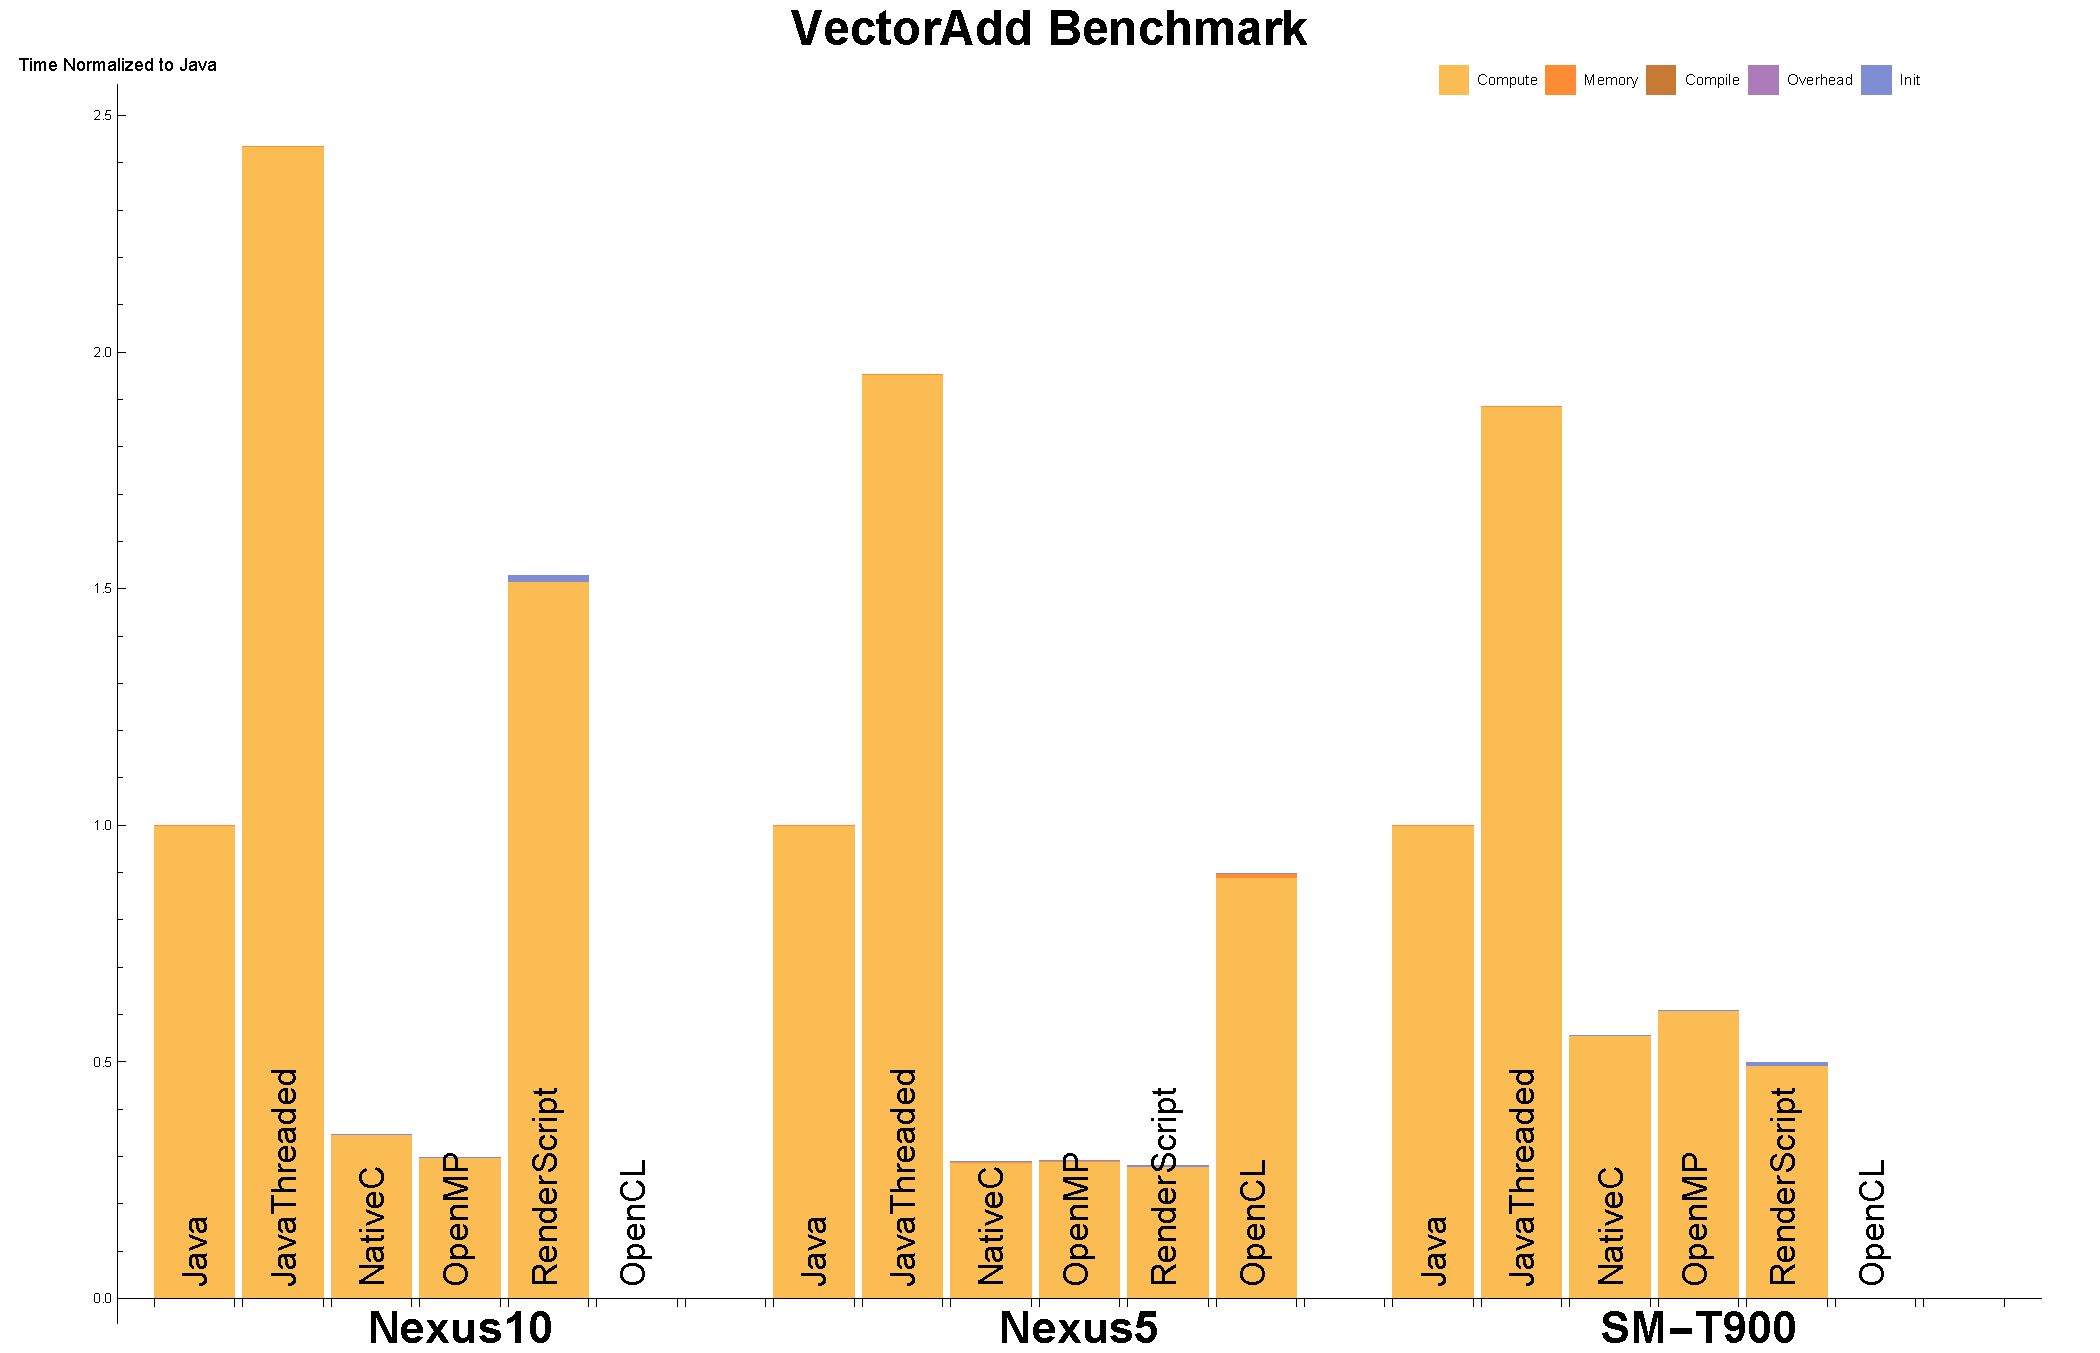
\includegraphics[width=\textwidth]{data/VectorAdd_onecompute_time.pdf}
      \caption{VectorAdd}\label{fig:vectoradd}
  \end{subfigure}
  \begin{subfigure}[b]{0.5\textwidth}
      \centering
      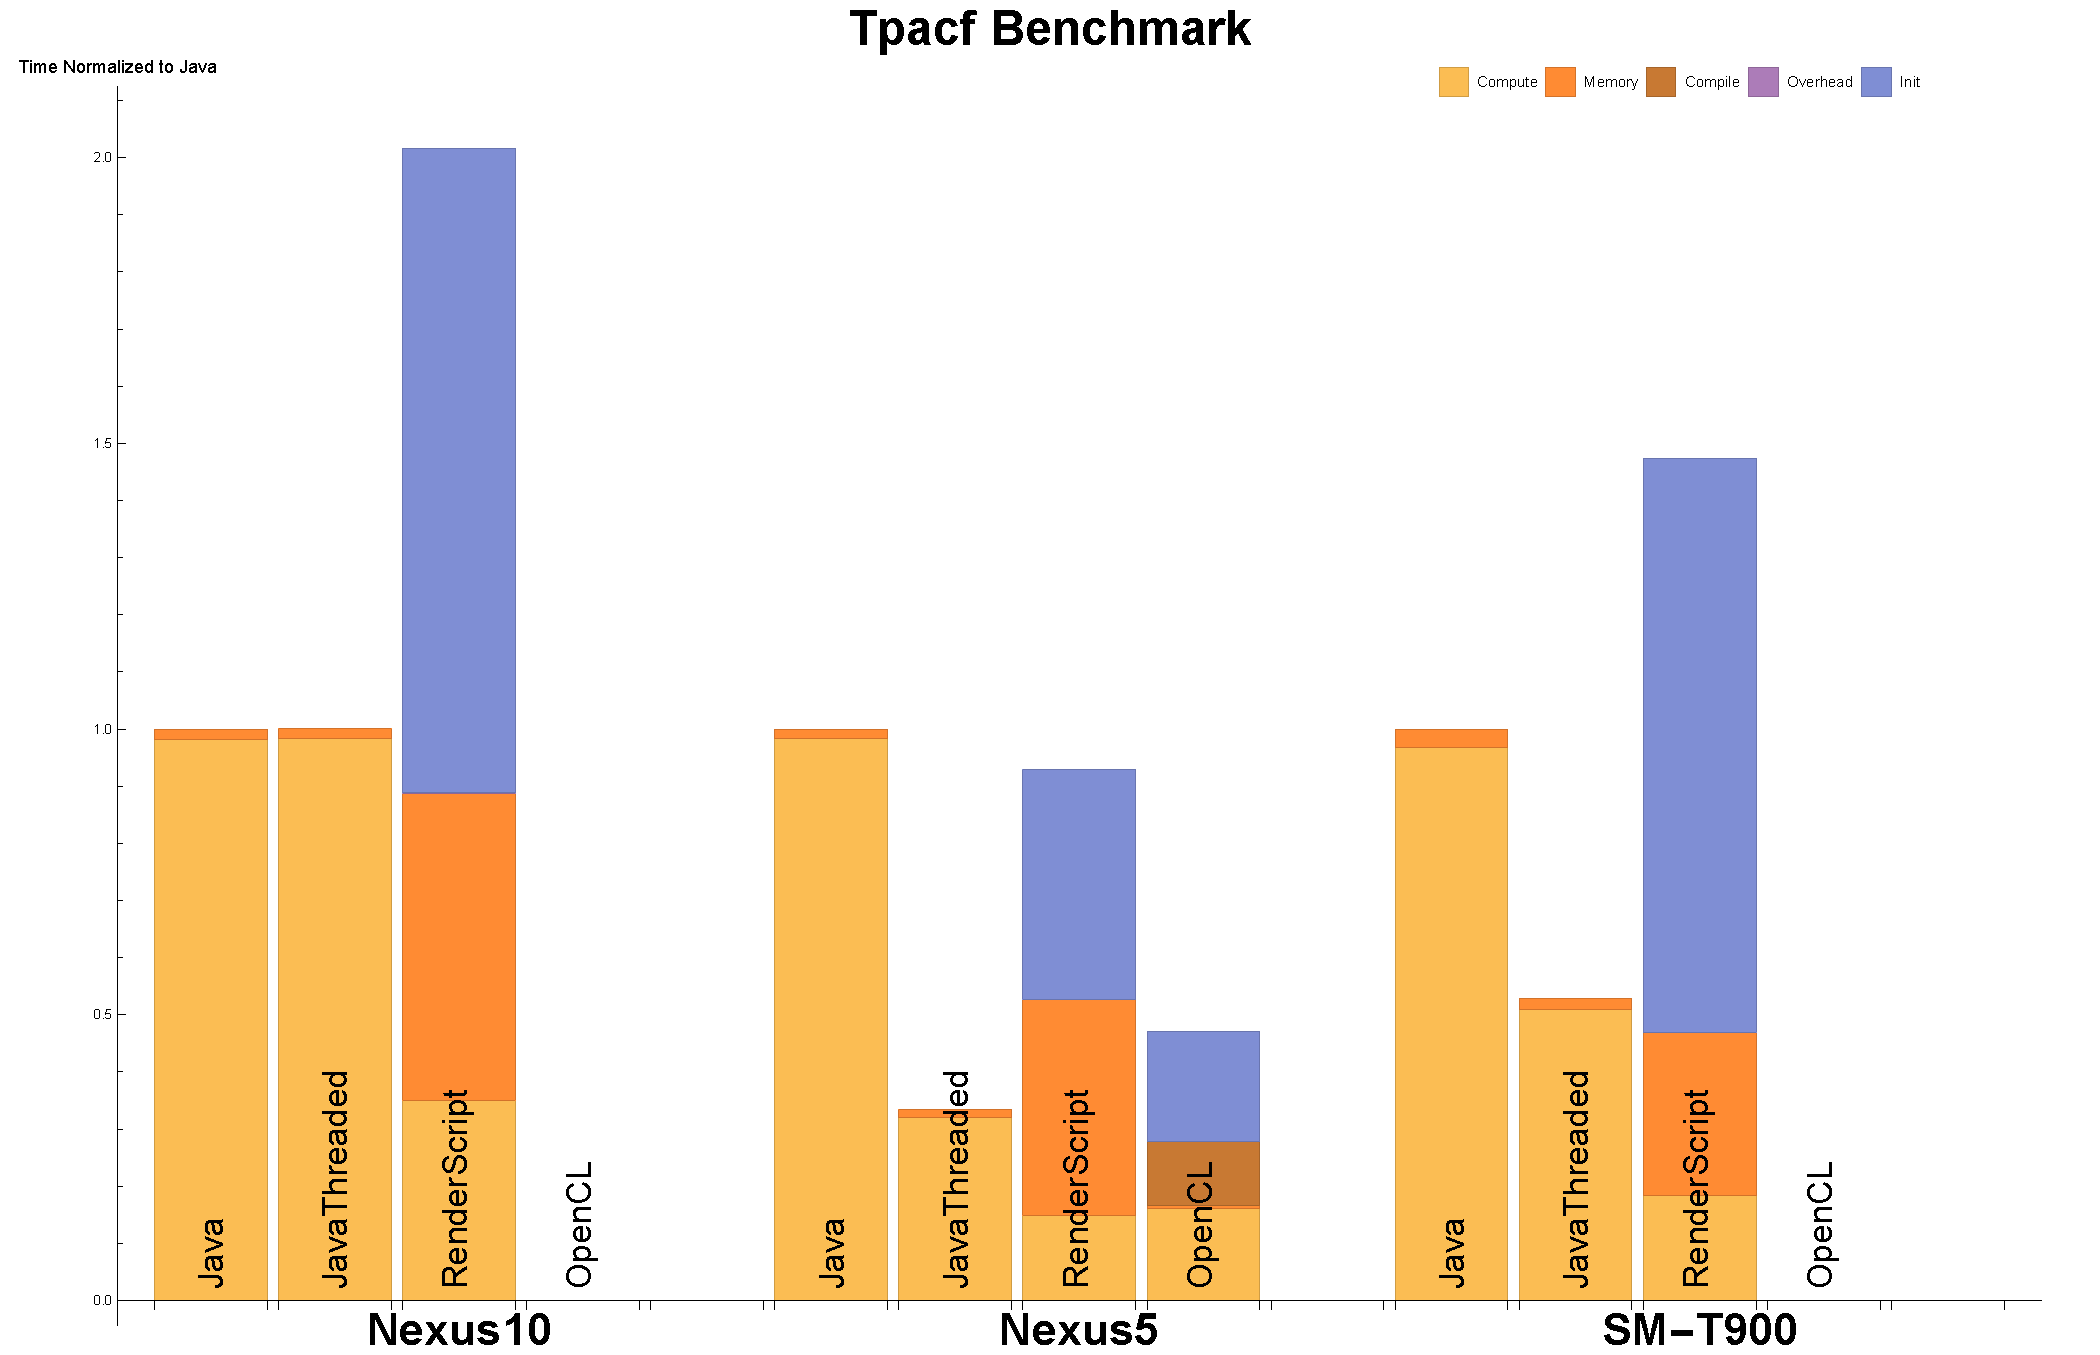
\includegraphics[width=\textwidth]{data/Tpacf_onecompute_time.pdf}
      \caption{TPACF}
      \label{fig:TPACF}
  \end{subfigure}

  \begin{subfigure}[b]{0.5\textwidth}
      \centering
      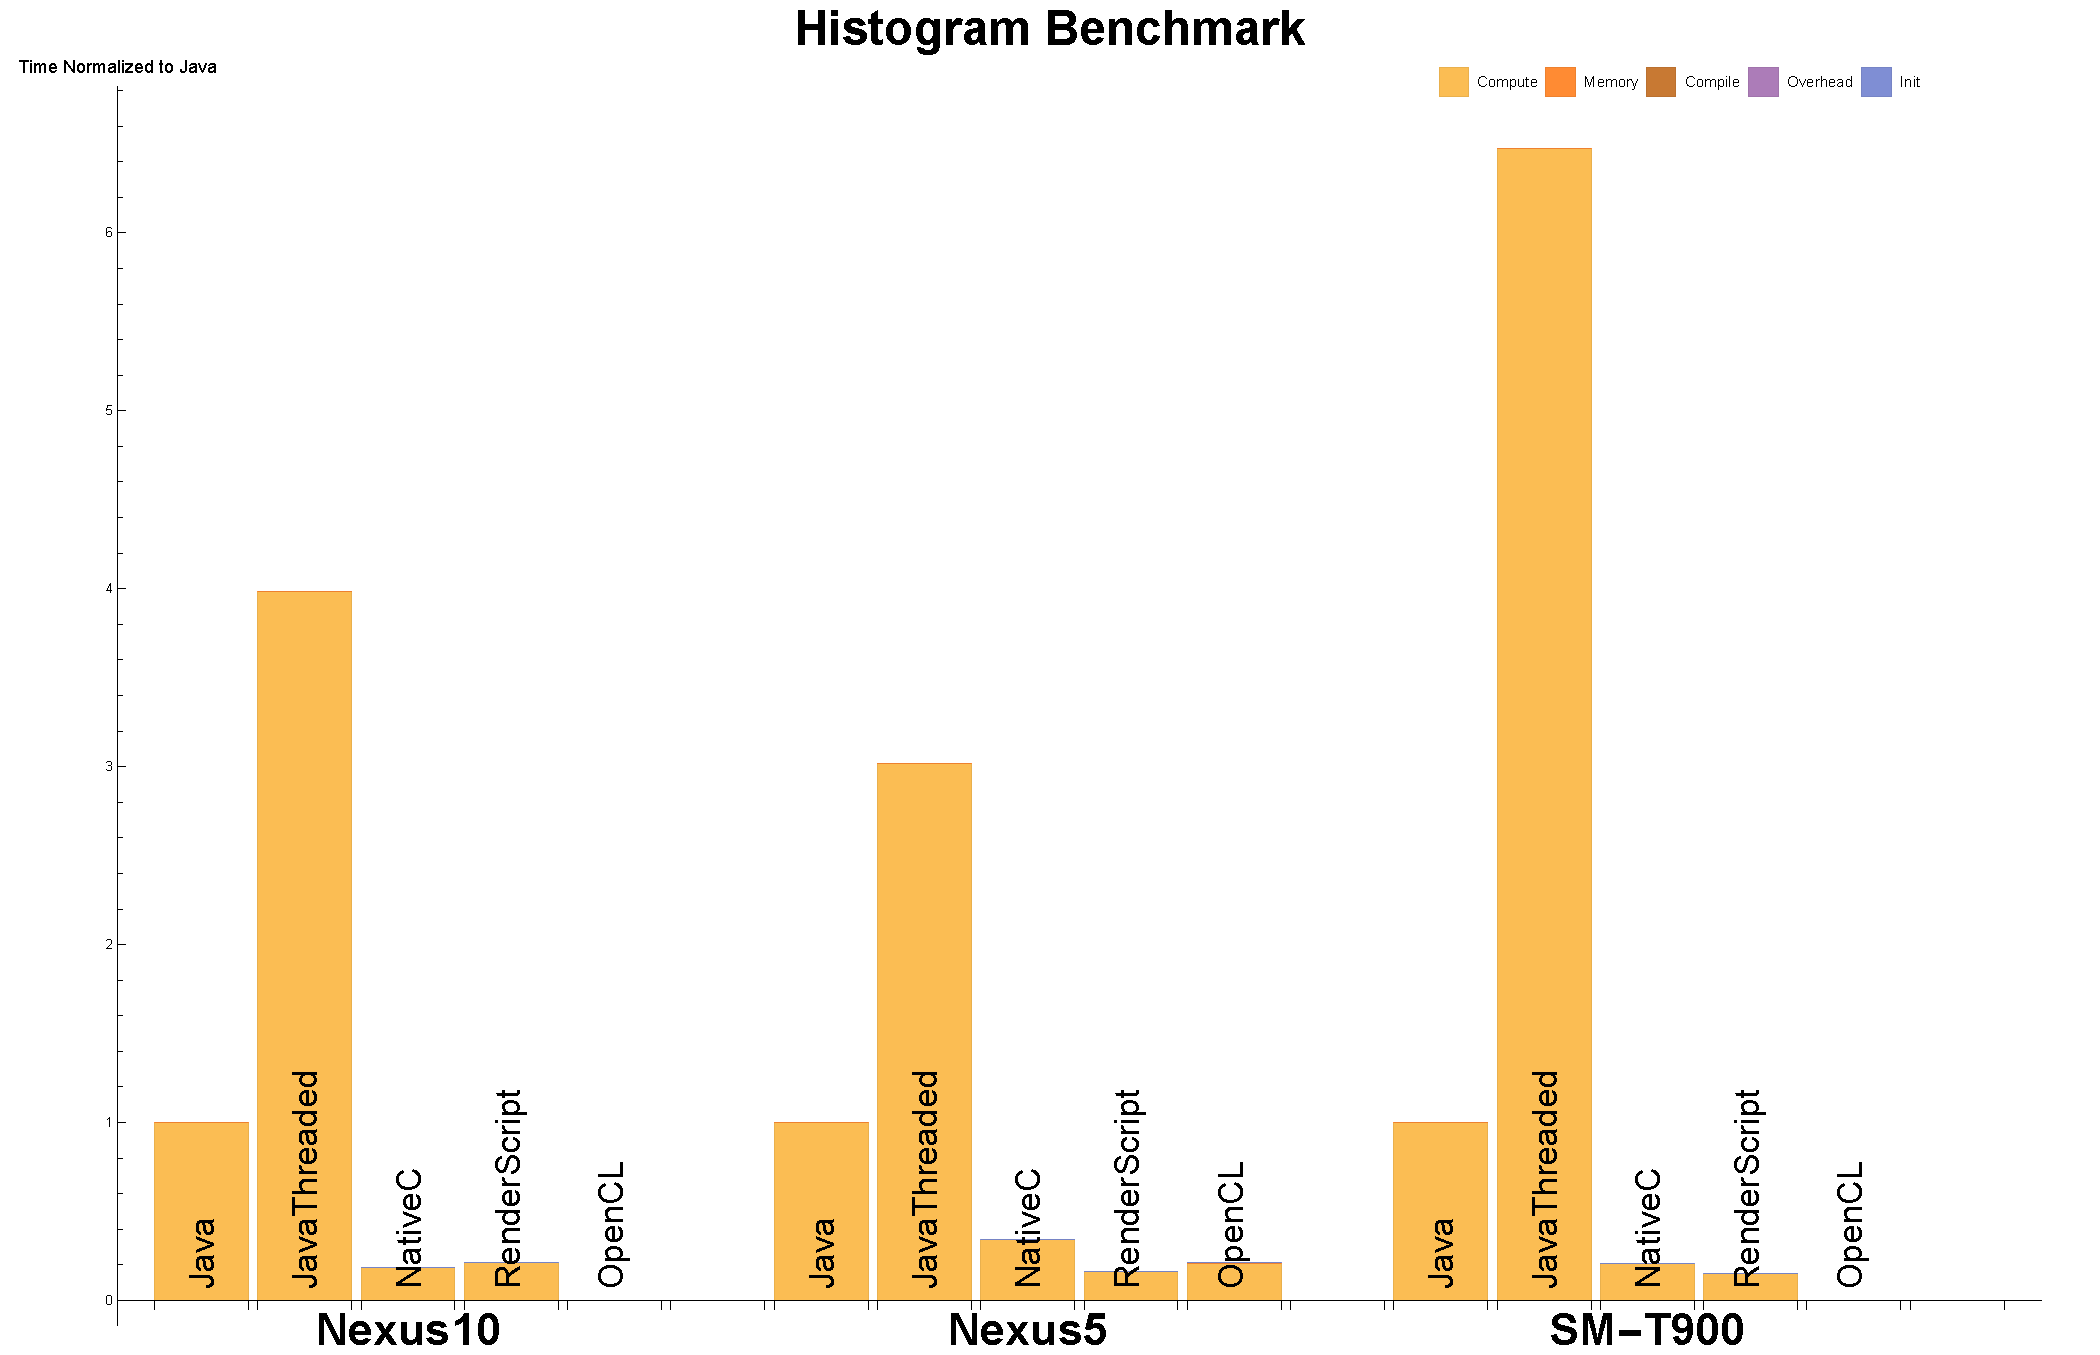
\includegraphics[width=\textwidth]{data/Histogram_onecompute_time.pdf}
      \caption{Histo}\label{fig:histo}
  \end{subfigure}
  \begin{subfigure}[b]{0.5\textwidth}
      \centering
      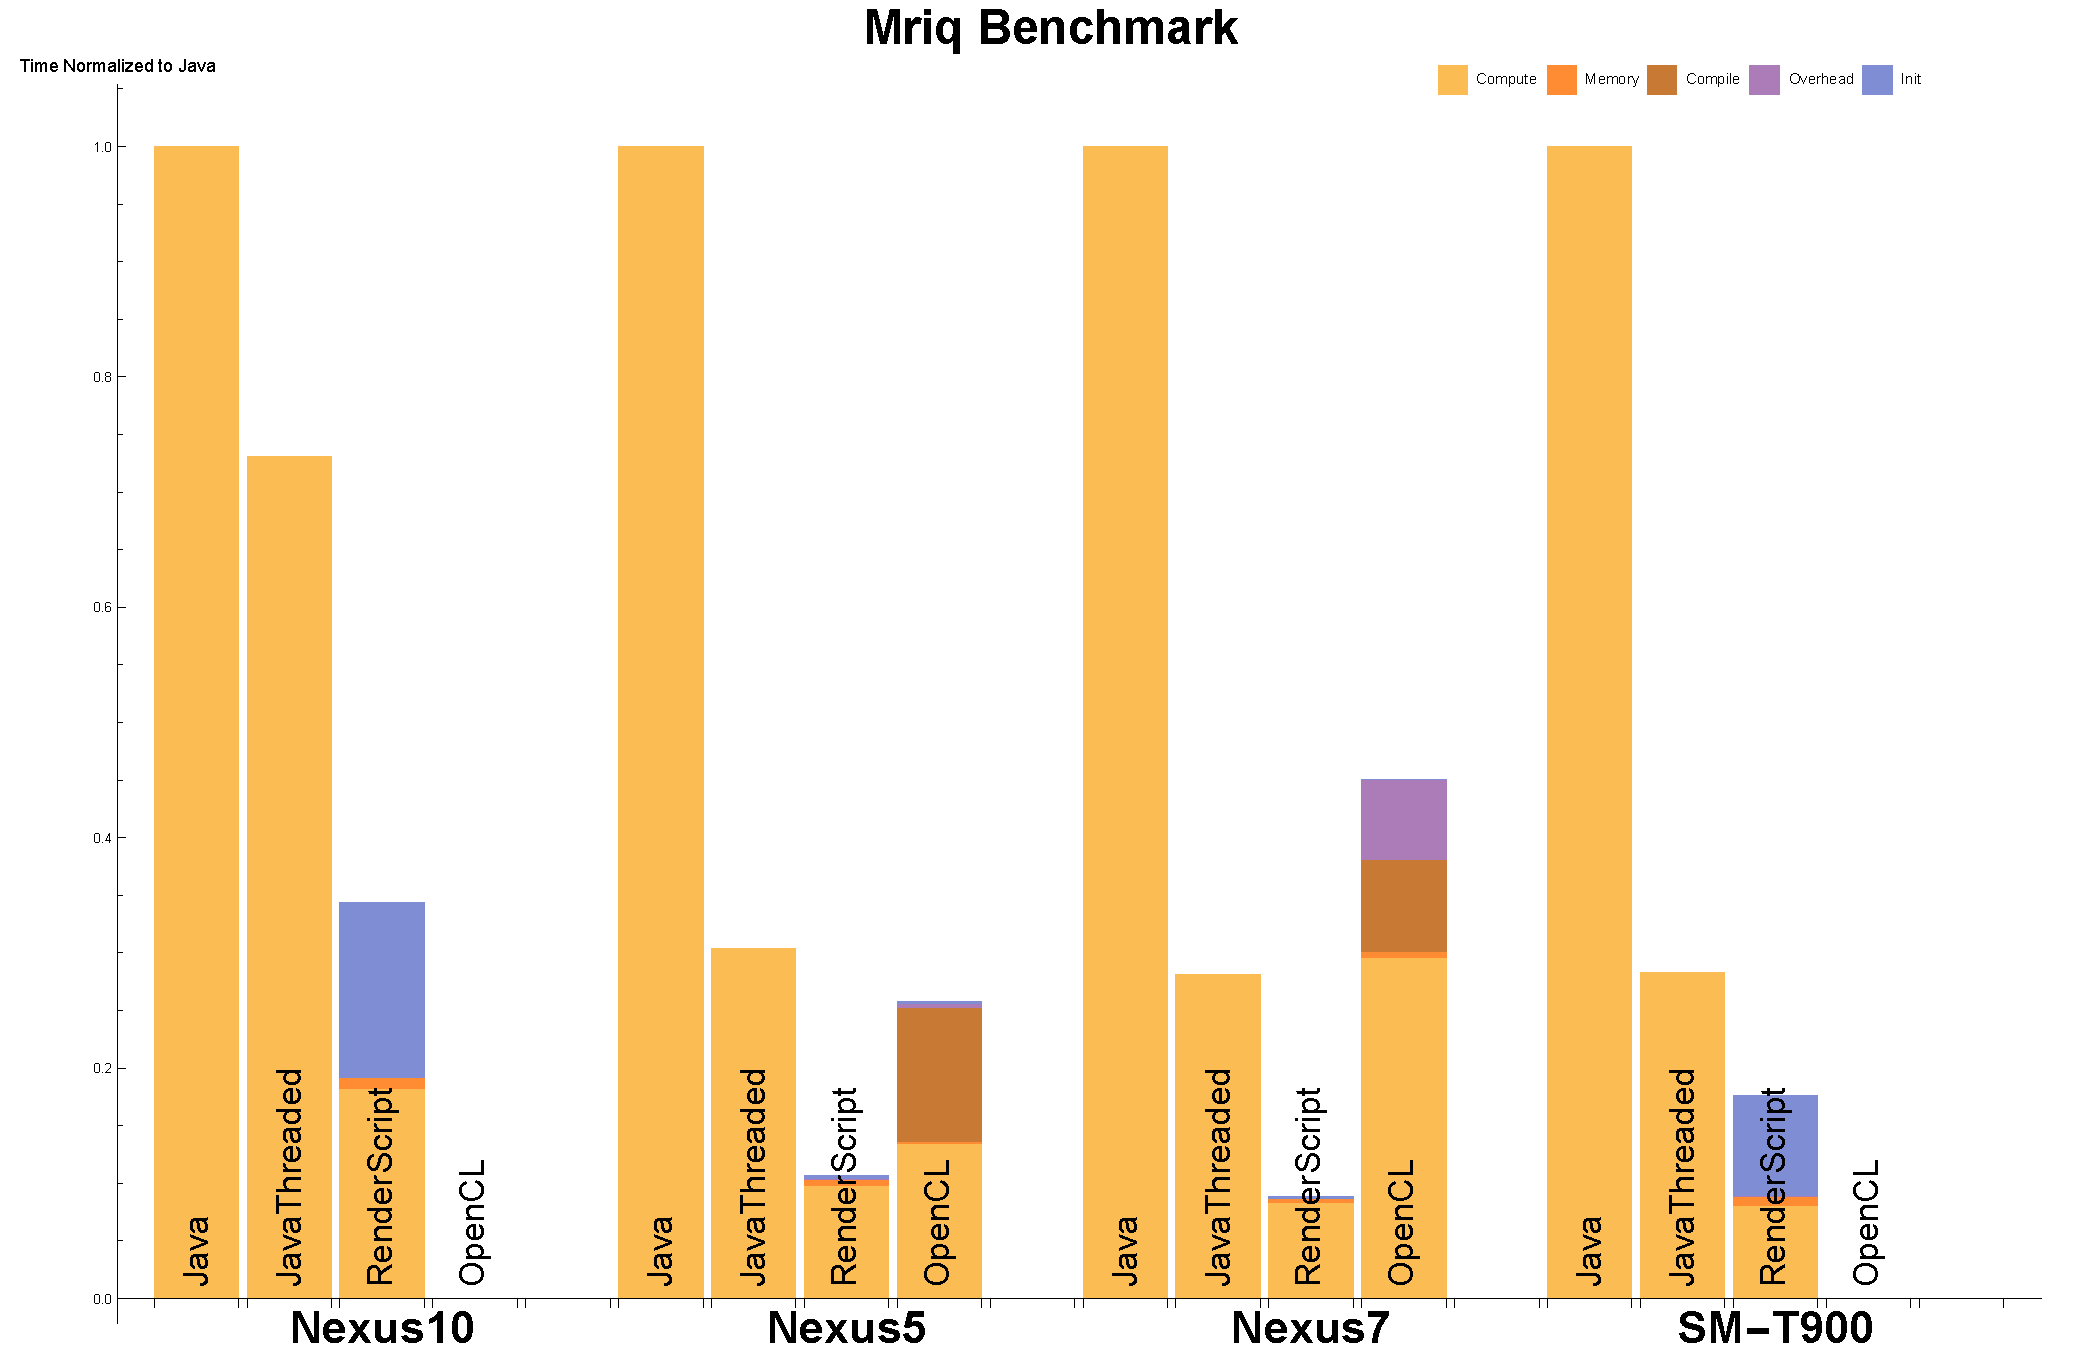
\includegraphics[width=\textwidth]{data/Mriq_onecompute_time.pdf}
      \caption{MRIQ}
      \label{fig:MRIQ}
  \end{subfigure}

  \begin{subfigure}[b]{0.5\textwidth}
      \centering
      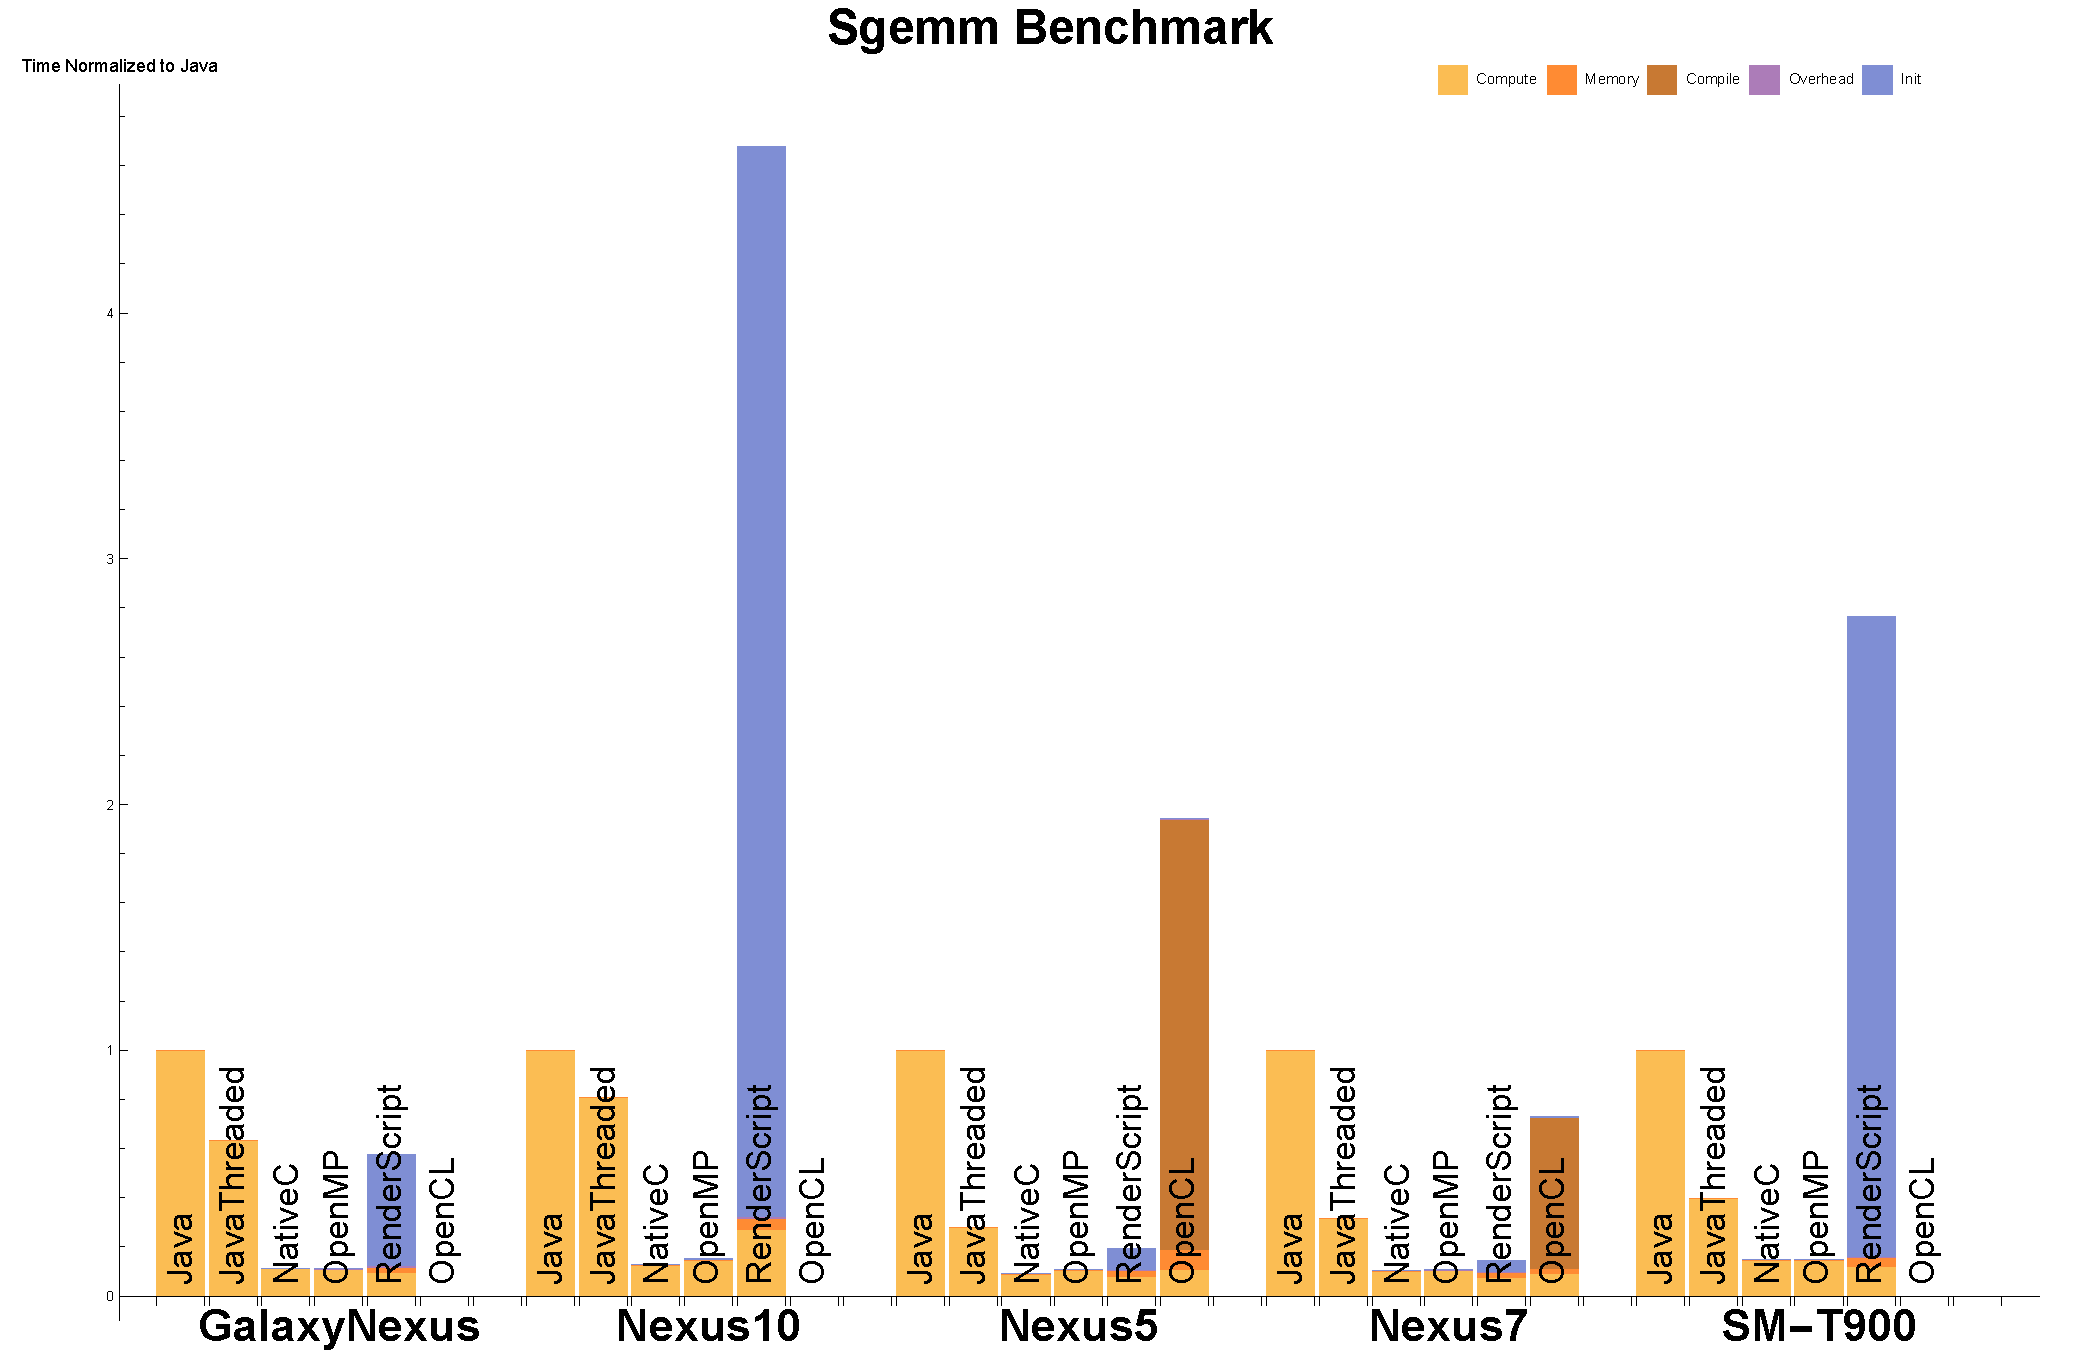
\includegraphics[width=\textwidth]{data/Sgemm_onecompute_time.pdf}
      \caption{Sgemm}\label{fig:Sgemm}
  \end{subfigure}
  \begin{subfigure}[b]{0.5\textwidth}
      \centering
      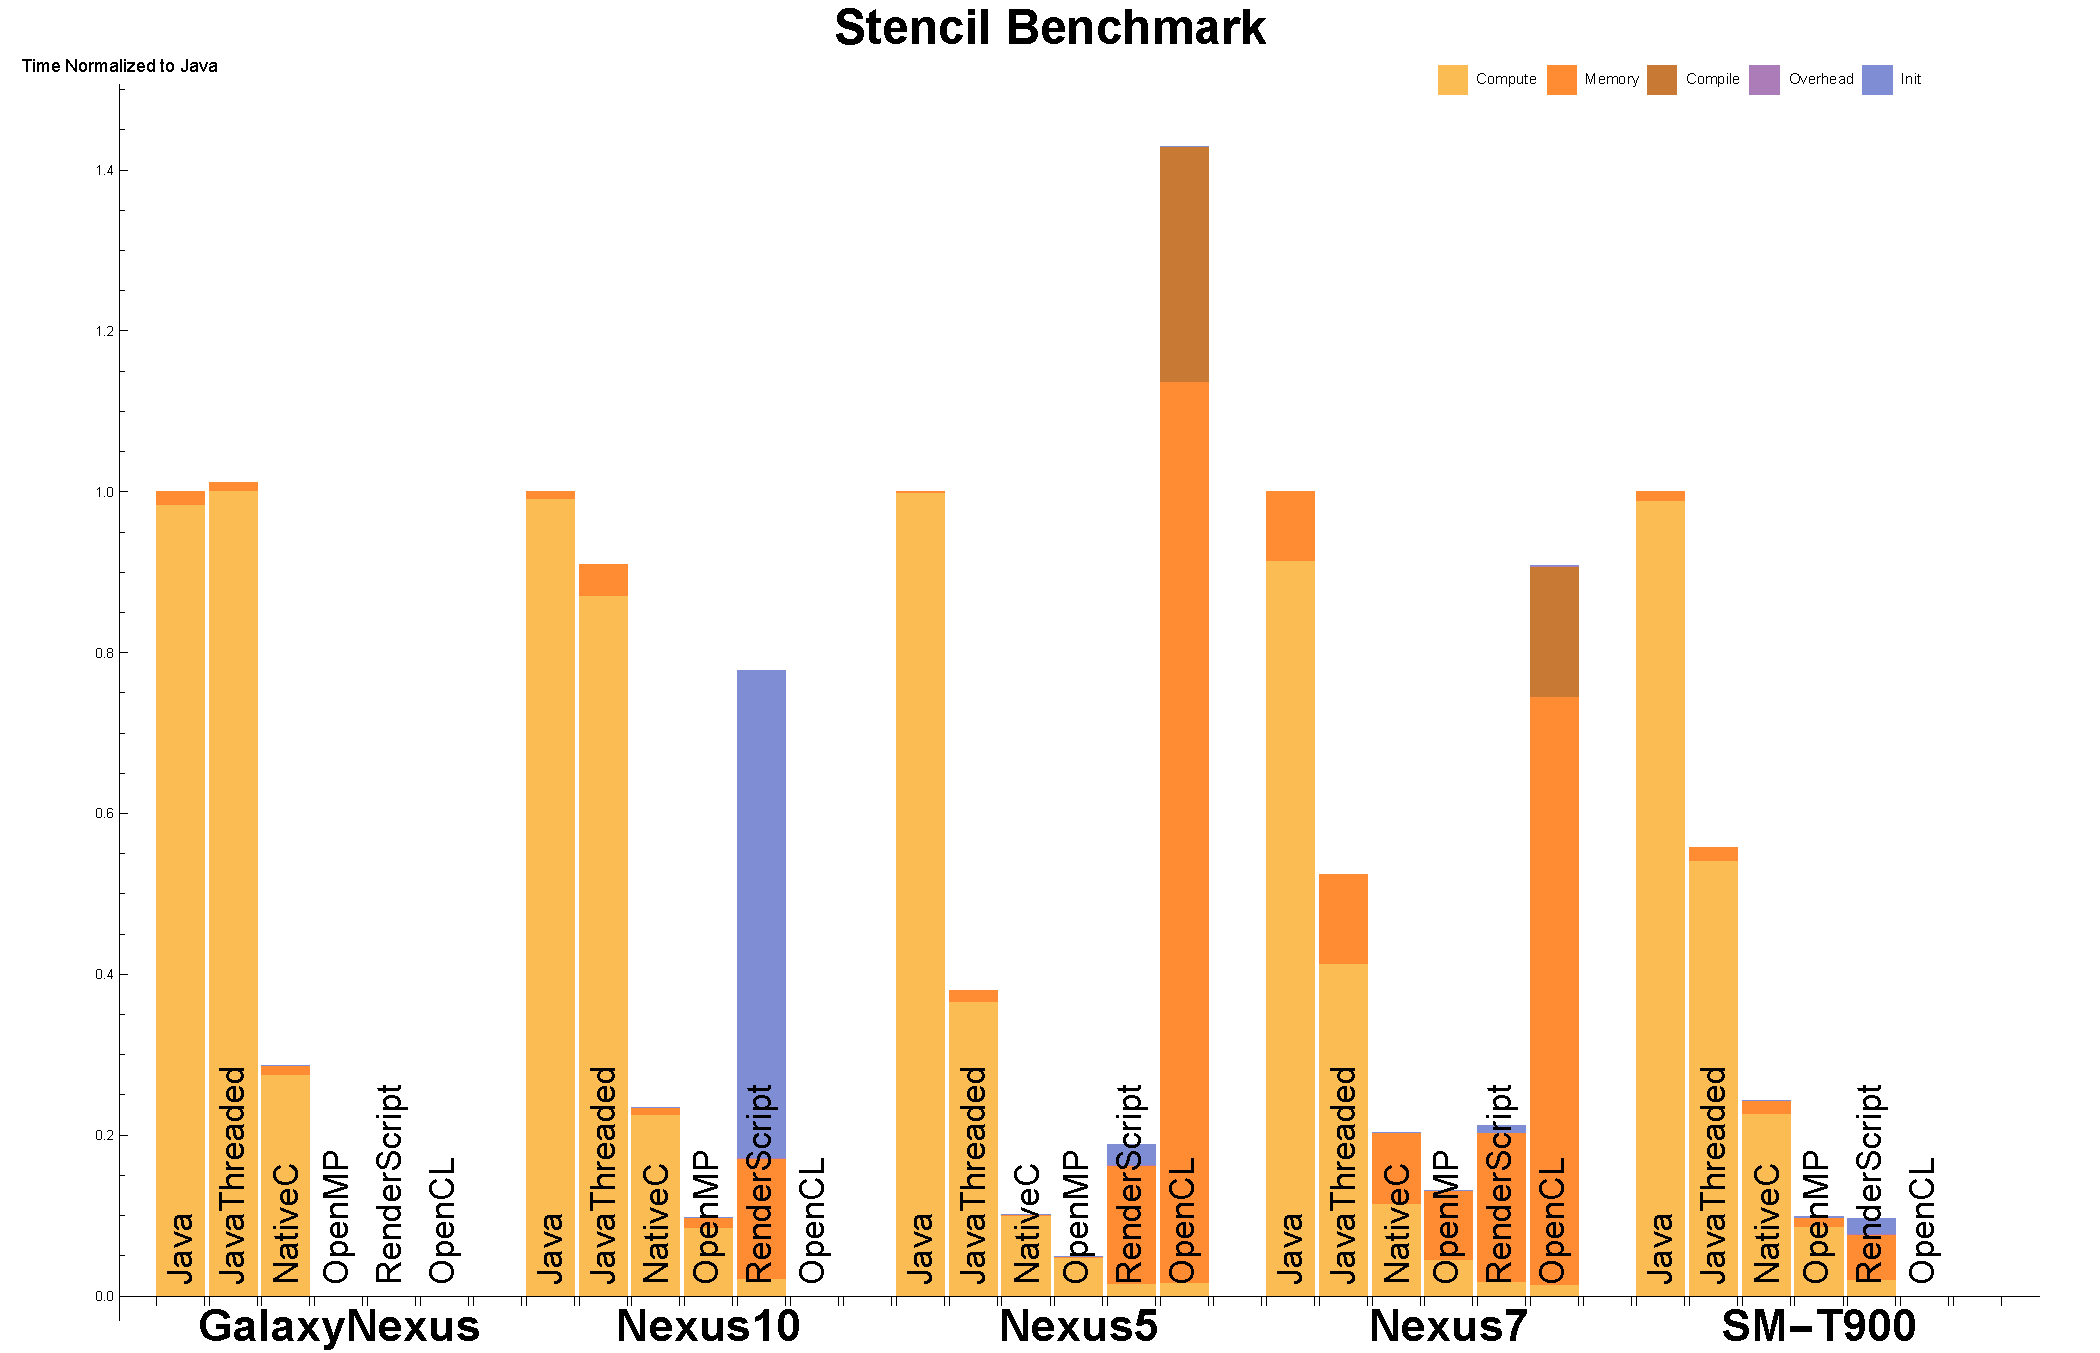
\includegraphics[width=\textwidth]{data/Stencil_onecompute_time.pdf}
      \caption{Stencil}
      \label{fig:Stencil}
  \end{subfigure}

  \caption{Runtime (one compute)}
\end{figure*}

We evaluate each benchmark and its implementations on the devices listed
  in Table~\ref{table:hardware}.
The performance measurments are collected by measuring the time
  spent within each section of the code (as discussed in~\ref{design}).
Each compute part of an implementation is run $5$ % TODO: what do we decide
  times and the minimum value is presented.
The performance times are also measured with the system connected to a
  power source, which avoids the device going to sleep.

\begin{figure*}[ht]
  \centering
  \begin{subfigure}[b]{0.95\textwidth}
      \centering
      
\includegraphics[width=\textwidth]{data/load_vectoradd_nexus5.pdf}
      \caption{VectorAdd}\label{fig:vectoradd}
  \end{subfigure}
  \begin{subfigure}[b]{0.95\textwidth}
      \centering
      
\includegraphics[width=\textwidth]{data/load_tpacf_nexus5.pdf}
      \caption{TPACF}
      \label{fig:TPACF}
  \end{subfigure}

  \begin{subfigure}[b]{0.95\textwidth}
      \centering
      
\includegraphics[width=\textwidth]{data/load_histogram_nexus5.pdf}
      \caption{Histo}\label{fig:histo}
  \end{subfigure}
  \begin{subfigure}[b]{0.95\textwidth}
      \centering
      
\includegraphics[width=\textwidth]{data/load_mriq_nexus5.pdf}
      \caption{MRIQ}
      \label{fig:MRIQ}
  \end{subfigure}

  \begin{subfigure}[b]{0.95\textwidth}
      \centering
      
\includegraphics[width=\textwidth]{data/load_sgemm_nexus5.pdf}
      \caption{Sgemm}\label{fig:Sgemm}
  \end{subfigure}
  \begin{subfigure}[b]{0.95\textwidth}
      \centering
      
\includegraphics[width=\textwidth]{data/load_stencil_nexus5.pdf}
      \caption{Stencil}
      \label{fig:Stencil}
  \end{subfigure}

  \caption{Load Nexus 5}
\end{figure*}


\begin{figure*}[ht]
  \centering
  \begin{subfigure}[b]{0.95\textwidth}
      \centering
      
\includegraphics[width=\textwidth]{data/load_vectoradd_nexus7.pdf}
      \caption{VectorAdd}\label{fig:vectoradd}
  \end{subfigure}
  \begin{subfigure}[b]{0.95\textwidth}
      \centering
      
\includegraphics[width=\textwidth]{data/load_tpacf_nexus7.pdf}
      \caption{TPACF}
      \label{fig:TPACF}
  \end{subfigure}

  \begin{subfigure}[b]{0.95\textwidth}
      \centering
      
\includegraphics[width=\textwidth]{data/load_histogram_nexus7.pdf}
      \caption{Histo}\label{fig:histo}
  \end{subfigure}
  \begin{subfigure}[b]{0.95\textwidth}
      \centering
      
\includegraphics[width=\textwidth]{data/load_mriq_nexus7.pdf}
      \caption{MRIQ}
      \label{fig:MRIQ}
  \end{subfigure}

  \begin{subfigure}[b]{0.95\textwidth}
      \centering
      
\includegraphics[width=\textwidth]{data/load_sgemm_nexus7.pdf}
      \caption{Sgemm}\label{fig:Sgemm}
  \end{subfigure}
%  \begin{subfigure}[b]{0.95\textwidth}
%      \centering
%      \includegraphics[width=\textwidth]{data/load_stencil_nexus7.pdf}
%      \caption{Stencil}
%      \label{fig:Stencil}
%  \end{subfigure}

  \caption{Load Nexus 7}
\end{figure*}



\subsubsection{Vector Add}

\subsubsection{SGEMM}

\subsubsection{Stencil}

\subsubsection{Histogram}

\subsubsection{CUTCP}


